\section{From a model to an agent}
\subsection{The parts of the system}

\begin{frame}{The pin factory coordinates the division of labor}
  \begin{center}
    \begin{minipage}{0.88\textwidth}
      \centering
      \large\itshape
      ``The greatest improvements in the productive powers of labour''
      grew from the division of labour.
    \end{minipage}

    \vspace{0.30em}
    {\footnotesize \citet[Book I, Chapter I]{smith1776wealth}.}

    \vspace{0.42em}
    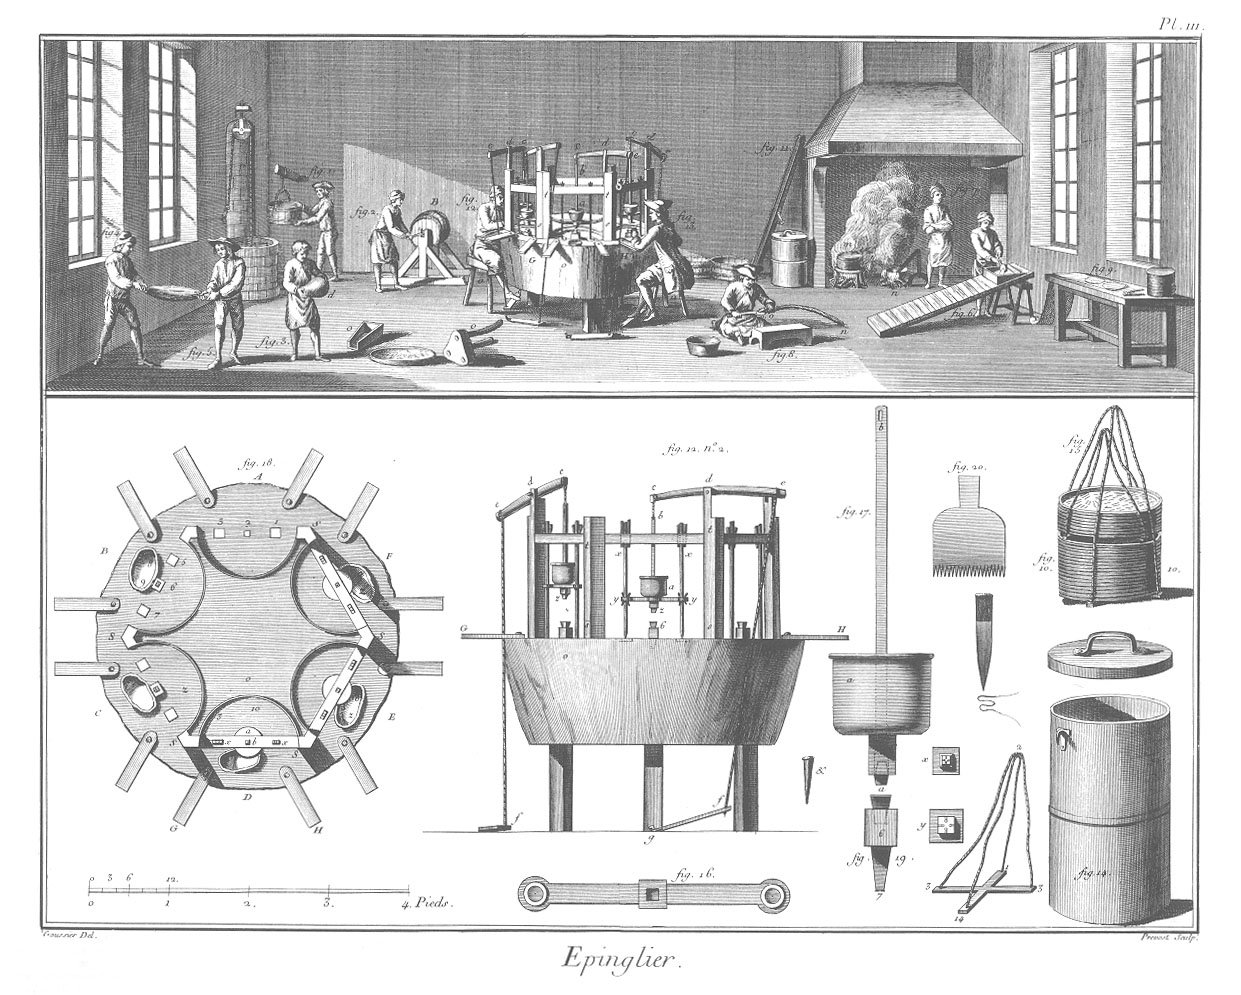
\includegraphics[width=0.78\textwidth,height=3.15cm,keepaspectratio,
      trim=0 275 0 0,clip]{figures/diderot-epinglier-1765.jpeg}

    \vspace{0.18em}
    {\scriptsize Diderot and d'Alembert, \emph{Encyclopédie},
    ``Épinglier,'' plate III (1765). Digital image: ARTFL Encyclopédie Project.}
  \end{center}

  \vfill
  Specialization raises output; \alert{coordination makes divided tasks one product.}

  {\scriptsize Pedagogical framing inspired by a teaching slide shared by Luis Garicano.}
\end{frame}

\begin{frame}{Delegation has a full cost}
  \begin{center}
    \large
    $\text{Net value of delegation}
    \;=\;
    \underbrace{\text{time saved}+\text{quality gain}}_{\text{benefit}}
    \;-\;
    \underbrace{\text{specification}+\text{verification}
      +\text{expected error cost}}_{\text{full cost}}.$
  \end{center}

  \vspace{0.65em}
  \begin{columns}[T,onlytextwidth]
    \column{0.48\textwidth}
      \begin{block}{A narrow calculation}
        The agent produces a WDI comparison in 20 minutes instead of 40.
      \end{block}
    \column{0.48\textwidth}
      \begin{block}{The complete workflow}
        Writing the request and checking definitions, years, revisions, and
        arithmetic require another 30 minutes.
      \end{block}
  \end{columns}

  \vfill
  ``The agent can do it'' does not establish that delegation improves the
  workflow. Count the handoff and review, not only production
  \citep{coase1937firm}.
\end{frame}

\begin{frame}{Knowledge is divided too}
  \begin{columns}[T,onlytextwidth]
    \begin{column}{0.47\textwidth}
      \begin{block}{Hayek: knowledge is dispersed}
        Relevant facts do not arrive in one complete bundle. People hold
        different knowledge of context, time, place, and purpose
        \citep{hayek1945knowledge}.
      \end{block}
    \end{column}
    \begin{column}{0.49\textwidth}
      \begin{block}{Garicano: route problems to knowledge}
        Routine problems can stay close to production; exceptional problems
        move to specialized problem solvers \citep{garicano2000hierarchies}.
      \end{block}
    \end{column}
  \end{columns}

  \vspace{0.65em}
  \begin{center}
  \begin{tikzpicture}[
    node distance=0.55cm,
    box/.style={draw=palegray,rounded corners=2pt,text width=3.15cm,
      minimum height=1.12cm,align=center,font=\small},
    arr/.style={-{Latex[length=1.8mm]},color=crimson,thick}
  ]
    \node[box] (student) {Student\\question + local context};
    \node[box,right=of student] (agent) {Agent\\routine production};
    \node[box,right=of agent] (expert) {Student + evidence\\exception + judgment};
    \draw[arr] (student)--node[above,font=\scriptsize]{work order}(agent);
    \draw[arr] (agent)--node[above,font=\scriptsize]{result + trace}(expert);
  \end{tikzpicture}
  \end{center}

  \vfill
  The student does not disappear from the workflow. The student supplies
  context, recognizes exceptions, and decides whether the answer can be kept.
\end{frame}

\begin{frame}{Checkpoint 2: Who knows what?}
  \alert{Block 1 · minutes 30--34}

  \vspace{0.55em}
  The WDI file and a ministry report give different under-five mortality values
  for the same country-year.

  \vspace{0.55em}
  Decide together:
  \begin{enumerate}
    \item What knowledge might each source hold that the other does not?
    \item What should the agent inspect, and what judgment remains with us?
  \end{enumerate}

  \vfill
  \begin{center}
    \textbf{2 minutes discuss} \hspace{2.0em} $\longrightarrow$ \hspace{2.0em}
    \textbf{2 minutes share}
  \end{center}
\end{frame}

\begin{frame}{AI includes several kinds of systems}
  \small
  \begin{tabularx}{\textwidth}{@{}>{\bfseries}p{3.0cm}X@{}}
    \toprule
    Term & Working definition for this course \\
    \midrule
    Artificial intelligence & A broad family of systems for prediction, perception, language, planning, or action. \\
    Large language model & A model that produces language, code, or a tool request from an instruction and context. \\
    Chat interface & A message window around a model. \\
    Coding agent & A model working in a loop with tools that can act inside a project. \\
    \bottomrule
  \end{tabularx}

  \vfill
  We use these terms separately because they imply different actions and
  different things to verify.
\end{frame}

\begin{frame}{From conversation to action}
  \small
  \begin{tabularx}{\textwidth}{@{}>{\bfseries}p{2.6cm}p{4.6cm}X@{}}
    \toprule
    Experience & Who executes & What we can observe \\
    \midrule
    Chat & A person copies, pastes, and runs each step. & A response. \\
    Code completion & A person works; the model suggests nearby code. & A code fragment. \\
    Agent & The system plans, uses tools, observes, and continues. & A sequence of actions. \\
    Coding agent & The agent operates on project files and the terminal. & Diffs, commands, logs, and artifacts. \\
    \bottomrule
  \end{tabularx}

  \vfill
  Codex and Claude Code are coding agents. Their project access allows them to
  read files, use tools, and return observable results
  \citep{openai2026codex,anthropic2025claudecode}.
\end{frame}

\begin{frame}{A coding agent is a system of parts}
  \begin{center}
  \begin{tikzpicture}[
    node distance=0.30cm,
    box/.style={draw=palegray,rounded corners=2pt,text width=2.10cm,
      minimum height=1.10cm,align=center,font=\small,inner sep=4pt},
    arr/.style={-{Latex[length=1.8mm]},color=crimson,thick}
  ]
    \node[box] (model) {Model\\language + code};
    \node[box,right=of model] (context) {Context\\files + history};
    \node[box,right=of context] (tools) {Tools\\editor + terminal};
    \node[box,right=of tools] (harness) {Harness\\loop + controls};
    \node[box,right=of harness] (human) {Person\\goal + judgment};
    \draw[arr] (model)--(context);
    \draw[arr] (context)--(tools);
    \draw[arr] (tools)--(harness);
    \draw[arr] (harness)--(human);
  \end{tikzpicture}
  \end{center}

  \vspace{0.75em}
  The harness connects the model to the environment and applies permissions. We
  still define the objective, the standard, and the final decision.
\end{frame}

\begin{frame}{Watch one tool-call loop}
  \begin{center}
  \begin{tikzpicture}[
    node distance=0.45cm,
    processbox/.style={draw=palegray,rounded corners=2pt,text width=2.6cm,
      minimum height=1.25cm,align=center,font=\small,inner sep=5pt},
    arr/.style={-{Latex[length=2mm]},color=crimson,thick}
  ]
    \node[processbox] (request) {\textbf{1. Request}\\Read a file or run a command};
    \node[processbox,right=of request] (permission) {\textbf{2. Permission}\\Is this action allowed?};
    \node[processbox,right=of permission] (execution) {\textbf{3. Execution}\\Ordinary software acts};
    \node[processbox,right=of execution] (observation) {\textbf{4. Observation}\\The result returns};
    \draw[arr] (request.east)--(permission.west);
    \draw[arr] (permission.east)--(execution.west);
    \draw[arr] (execution.east)--(observation.west);

    \coordinate (return-right) at ($(observation.south)+(0,-0.62cm)$);
    \coordinate (return-left) at ($(request.south)+(0,-0.62cm)$);
    \draw[arr]
      (observation.south)--(return-right)--
      node[below,font=\scriptsize,text=darkgray] {If another action is needed, the loop begins again.}
      (return-left)--(request.south);
  \end{tikzpicture}
  \end{center}

  \vfill
  This loop helps us ask what actually happened. Evidence of an action comes
  from the exposed tool call, result, or log.
\end{frame}

\begin{frame}{Four course tools, four jobs}
  \footnotesize
  \renewcommand{\arraystretch}{1.18}
  \begin{tabularx}{\textwidth}{@{}>{\bfseries}p{1.7cm}p{5.2cm}X@{}}
    \toprule
    Tool & What it does & Decision left to the analyst \\
    \midrule
    R & Runs data and statistical operations. & Whether an operation represents the intended concept. \\
    RStudio & Keeps scripts, console, files, objects, and plots visible. & Whether the code is substantively correct. \\
    Quarto & Combines code, prose, and output in an optional notebook. & Whether the narrative follows from the evidence. \\
    Codex & Reads, proposes, edits, runs, and checks inside a project. & Whether its output deserves our trust. \\
    \bottomrule
  \end{tabularx}
\end{frame}

\subsection{Choose the task first}

\begin{frame}{Choose the tool after the task}
  \small
  \begin{tabularx}{\textwidth}{@{}p{4.0cm}p{4.2cm}X@{}}
    \toprule
    Need & Smallest useful system & Acceptance evidence \\
    \midrule
    Calculate a summary & R script & A hand check and a reproducible result \\
    Explain an error & Chat or agent with the error and code & Explanation matches a small test \\
    Modify a project & Coding agent with limited access & Diff, clean run, and relevant checks \\
    Decide a policy interpretation & Person with evidence & Definitions, assumptions, and argument \\
    \bottomrule
  \end{tabularx}

  \vfill
  More autonomy creates more places where something can go wrong. Start with the
  simplest system that lets you verify the result.
\end{frame}

\begin{frame}{Checkpoint 3: Choose the smallest system}
  \alert{Block 1 · minutes 46--50}

  \vspace{0.55em}
  Before comparing mortality across years, you need to know whether the
  indicator's definition or unit changed.

  \vspace{0.55em}
  Decide together:
  \begin{enumerate}
    \item Which is the smallest useful system: R, chat, a coding agent, or a person?
    \item What evidence would let you accept its answer?
  \end{enumerate}

  \vfill
  \begin{center}
    \textbf{2 minutes discuss} \hspace{2.0em} $\longrightarrow$ \hspace{2.0em}
    \textbf{2 minutes share}
  \end{center}
\end{frame}
